
% ===============================================================
% =						System Description						=
% ===============================================================
\chapter{System Description and Functionalities}
\label{cha:system}
This chapter describes the architecture and general structure of the system, as well as a detailed explanation about the functionalities implemented with the proposed technologies and interface displayed.

\section{System Description}
\label{sec:system_description}


\section{Functionalities}
\label{sec:functionalities}

This section describes in detail the functionalities and experiments implemented in our system. The set of functionalities implemented were considered to be more interesting to explore in a real-time environment than the usual set of features already presented in regular camera applications or digital cameras.

\subsection{Face Detection and Composition Guidelines}
\label{sub:face_guidelines}



\subsection{Colour Templates and Hue Counting}
\label{sub:color}


\subsection{Colour Histograms and Average Saturation}
\label{sub:histograms}

\subsection{Object Segmentation}
\label{sub:segmentation}

Unless it is a photography of a seascape or a landscape, it is normal for a photo to have a relevant subject. With this in mind, segmentation of a subject in multiple scenarios might be useful to attain a better composition.

Segmentation of an object in a photo, is a topic that as already been widely researched. One of the simplest ways of extracting information about the object in a real-time scenario is to have information about its background beforehand and subtract. 

In \cite{yang2004real}, \citeauthor{yang2004real} describe a system for security cameras, able to recognize and tracking a moving object. This is possible once the system is collecting information about the background as time passes. Using the information about the background, the system can subtract any object that considers strange to the background, and start the tracking. This method as the advantage of being fast and discard the possibility of training a classifier for object identification. 
\citeauthor{butler2003real} describe a similar approach in \cite{butler2003real}, where the key is to learn the background and generate a model of it by representing each pixel in the frame by a group of clusters, where these clusters are ordered by the likelihood of modelling the background. Incoming pixels are matched against the corresponding cluster group and classified as part of the background.
In our case, these methods have an obvious problem. Normally, the subject its already placed when the user wants to take a photo, therefore, the subject would be confused as a background or, the user would have to point the camera before placing the subject to initiate a process of extracting information and learn what's the background. When talking about a  camera in a mobile device or any digital camera, this method is nearly impractical, as the regular user tends to move the arms quite easily ruining the learning process started before. Thus, being an unreliable method for object segmentation.

For our use case, we envision a method for generic object segmentation that could be used in real-time. Since it is for generic objects, we couldn't train a classifier to recognize multiple objects, or use edges information for comparison, as it would need multiple photos for data collection, and the segmentation would be limited to a few objects. 

\subsubsection{Algorithm Description}

As mentioned in \cite{Santos} and \cite{kamps2012rules}, colour is a very important feature in a photo. With this in mind, when photographing, the main subject should cause visual impact due to its contrast relative to the background or other elements in the scenery. For this, we used a slightly simplified version of the \emph{Histogram Based Contrast} (HC) method described by \citeauthor{cheng2011global} in \cite{cheng2011global} for extraction of salient regions in a photo that evaluates global contrast differences, calculating saliency values for image pixels using color statistics. The saliency of a pixel is defined using its color contrast to all other pixels in the image. This can be described as,

\begin{equation}
S(I_{k}) = \sum_{\forall I_{i} \in I} D(I_{k}, I_{i}),
\end{equation}

where $D(I_{k}, I_{i})$ is the color distance between saliency value $I_{k}$ and pixel $I_{i}$ in the input image in the \emph{L*a*b*} color space. Since this computationally expensive, \citeauthor{cheng2011global}, reduces the number of colors needed to consider, by quantizing each color channel to have 12 different values, reducing the number of colors to $12^{3} = 1728$. Since a natural image covers only a small portion of the full color space, the less occurring colors are ignored, ensuring that the most occurring ones, cover at least 95\% of the image pixels. The remaining 5\% are replaced by the closest colors in the histogram. Since this quantization might introduce artifacts, the author preforms a smoothing procedure over each saliency value. Each saliency value is replaced by the weighted average of the $n/4$ neighbours where $n$ is the number of colors that fill 95\% of the image pixels.

After obtaining a saliency map, the map is turned into a binary segmentation mask using a fixed threshold. Finally GrabCut\cite{rother2004grabcut} will be used repeatedly to refine the segmentation result initially obtained by the binary segmentation mask.

\subsubsection{Implementation Details}

To use this algorithm in a real-time scenario in a mobile device, our implementation had to be more simplified with little changes. GrabCut is too heavy to run smoothly on a mobile device, and for that reason, we had to discard its usage sacrificing the refinement of the segmentation for speed. After obtaining the saliency map described in \cite{cheng2011global}, we give a label to each pixel depending on its value. These labels would be used in GrabCut to define which pixels are considered foreground, probable foreground, background, or probable background. In our case, we used the labels to create masks with the areas defined as probable foreground and probable background.
We defined experimentally the thresholds, classifying a pixel as probable foreground if its value was bigger or equal to 200 and probable background if it was between 20 and 200.

After obtaining a mask with each pixel labelled, we created a mask with all pixels that were considered as probable foreground and calculated the center of mass for the resulting mask. To remove artifacts that might exist from using an incorrect threshold value, generate a bounding rectangle that starts at the center of mass calculated and expands in every direction. Each edge will continue expanding while each row or column that passes, has at least a count of 25 pixels belonging to the segmentation mask, and stops when 50 rows or columns have been covered with a count of pixels bellow the previously stated. These thresholds were found experimentally and seem reasonable for the test images.

Obtained the bounding rectangle and mask with areas considered probable foreground, we had a good estimate of what was the main object in the scenario. The result of the segmentation was a section of the mask containing the probable foreground pixels, cropped in the area defined by the bounding rectangle. Since this algorithm is not sensitive to slight variations in lightning, we merged the probable foreground pixels with the probable background ones and cropped with the bounding rectangle. This would later be helpful filling the gaps in the mask, as this algorithm was not sensitive to slight light changes.

\subsubsection{Interface Display}

Generated the mask we chose to simply show a semi-transparent mask over the live feed obtained from the camera, as shown in Figure \ref{fig:interface_segmentation}. This would be a good indicator of what as the subject in the scenario and if it had any color striking features relatively to the rest of the elements.

\begin{figure}[htbp]
	\centering
	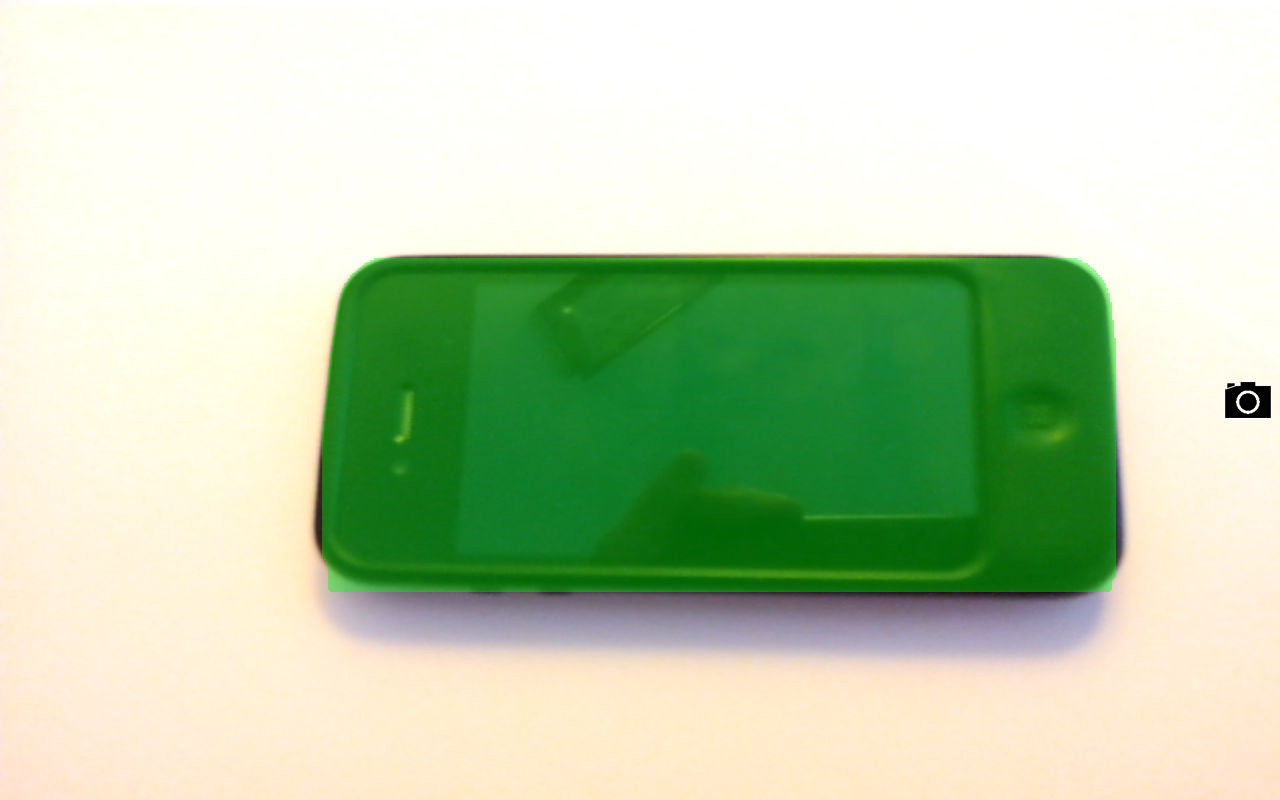
\includegraphics[scale=0.2]{interface/interface_segmentation.png}
    \caption{Example of object segmentation interface. The resulting mask of the algorithm is then displayed as a green overlay in the camera live feed.}
  	\label{fig:interface_segmentation}
\end{figure}

This could also be used together with guideline such as Rule of Thirds, described in \ref{sub:face_guidelines}, to reposition the object and change the composition.

\subsubsection{Discussion}

Being an incomplete algorithm, it does not work perfectly. Since it depends on the global contrast of a subjects colours, this segmentation might not work if the background is not plain or simple. Even with slight camera shake, this algorithm can extract the subject quite effectively. Figure \ref{fig:seg_example} show the multiple stages taken to segment an object in an image and its final result.

\begin{figure}[htbp]
	\label{fig:seg_example}	
	\hspace*{-20pt}
    \begin{tabular}{cccccccc}
    	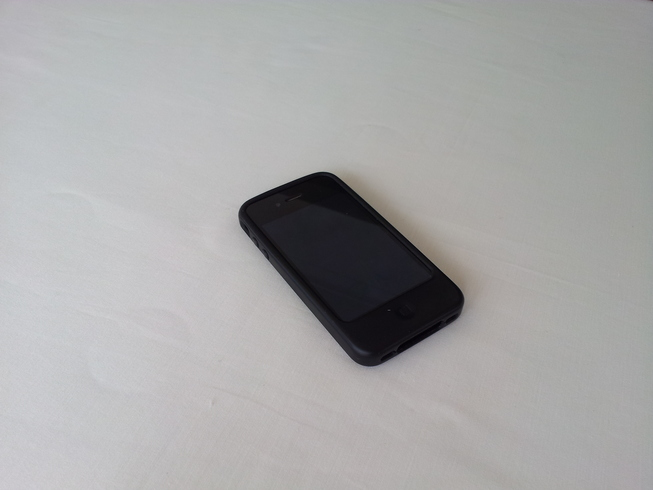
\includegraphics[width=0.14\textwidth]{interface/segmentation/3/re_3.jpg}        &
		\hspace*{-13pt}    	
    	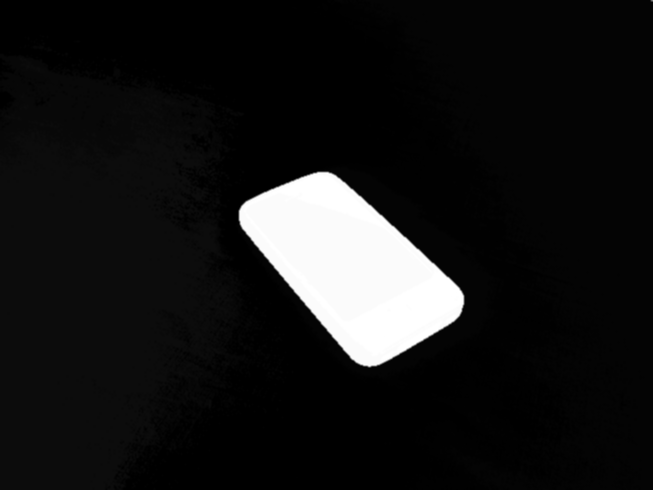
\includegraphics[width=0.14\textwidth]{interface/segmentation/3/re_3_sal.png}    & 						\hspace*{-13pt}
    	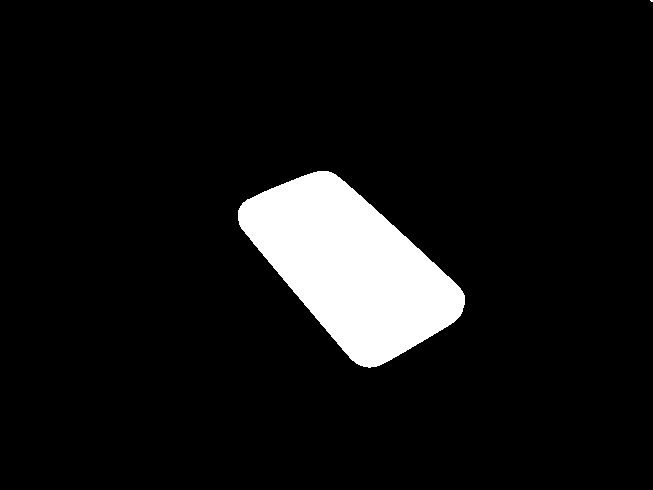
\includegraphics[width=0.14\textwidth]{interface/segmentation/3/re_3_bmask.png}    & 					\hspace*{-13pt}
    	
\includegraphics[width=0.14\textwidth]{interface/segmentation/3/re_3_pr_bgd.png}    & 					\hspace*{-13pt}
		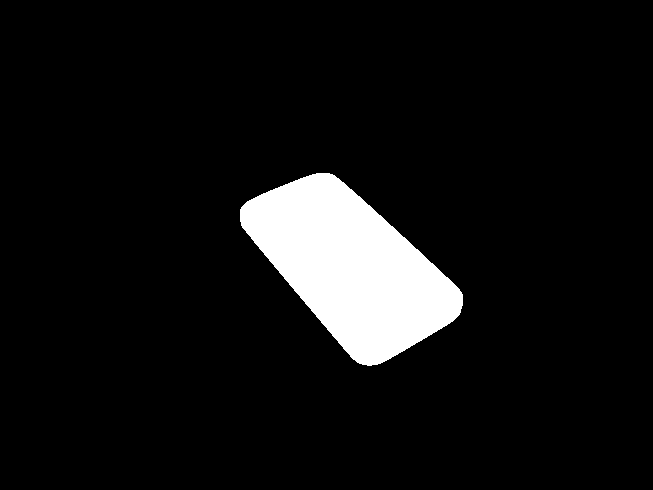
\includegraphics[width=0.14\textwidth]{interface/segmentation/3/re_3_pr_fgd.png}    & 					\hspace*{-13pt}
		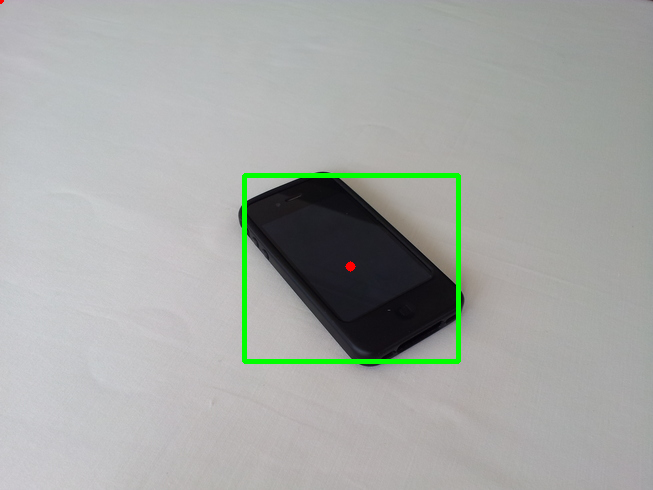
\includegraphics[width=0.14\textwidth]{interface/segmentation/3/re_3_rect.png}    & 					\hspace*{-13pt}
		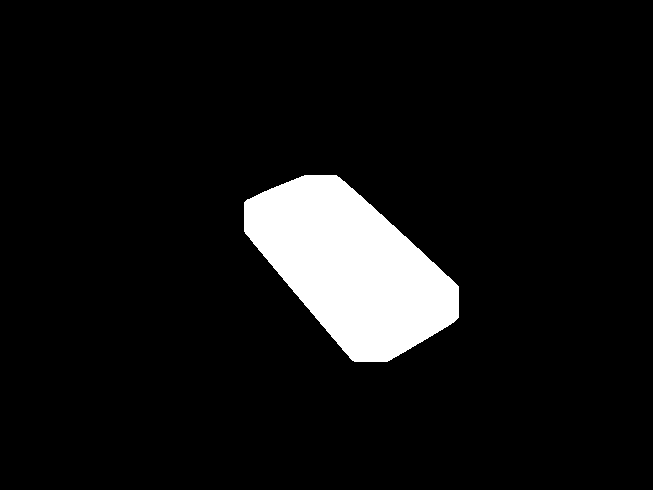
\includegraphics[width=0.14\textwidth]{interface/segmentation/3/re_3_mask.png}    & 					\hspace*{-13pt}
		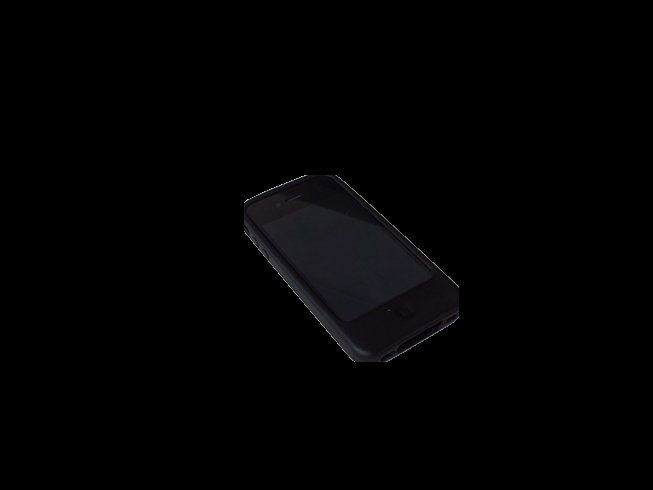
\includegraphics[width=0.14\textwidth]{interface/segmentation/3/re_3_seg.png} \\
    
    	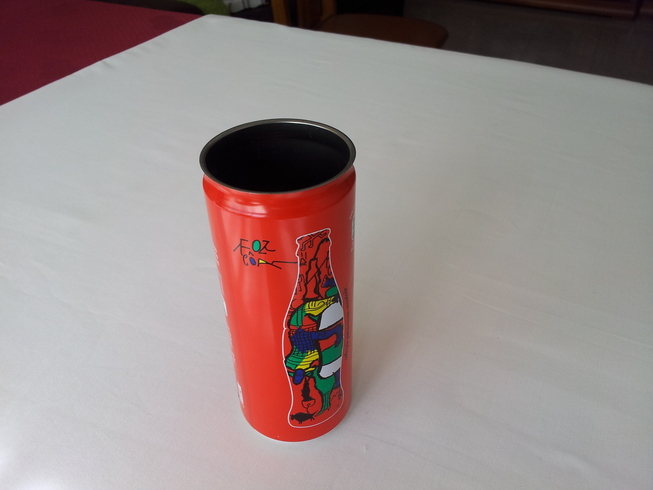
\includegraphics[width=0.14\textwidth]{interface/segmentation/2/re_2.jpg}    & 							\hspace*{-13pt}
		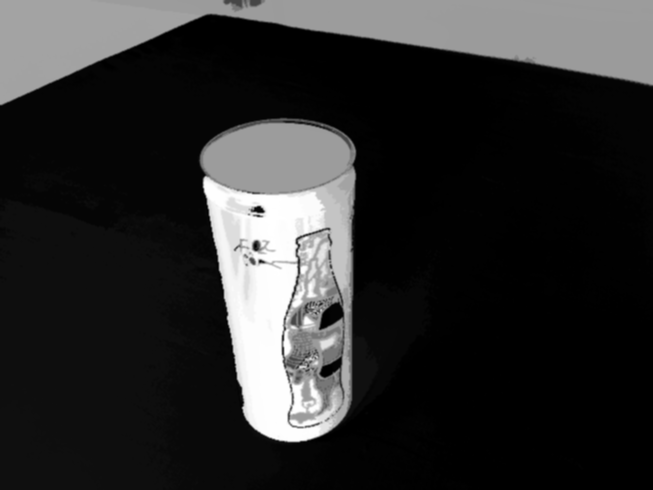
\includegraphics[width=0.14\textwidth]{interface/segmentation/2/re_2_sal.png}    & 						\hspace*{-13pt}
		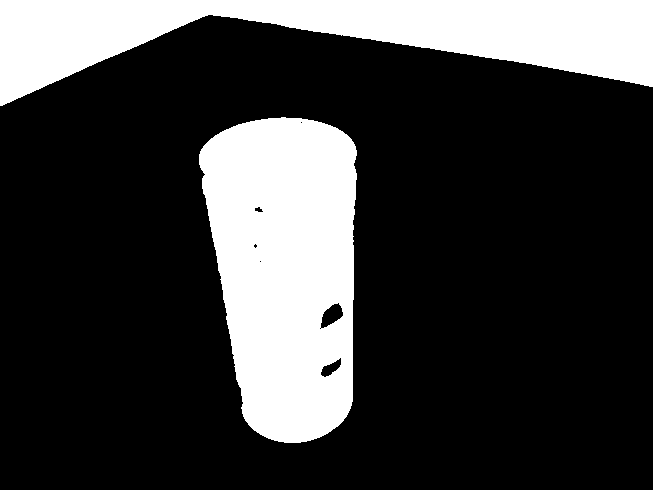
\includegraphics[width=0.14\textwidth]{interface/segmentation/2/re_2_bmask.png}    & 					\hspace*{-13pt}
		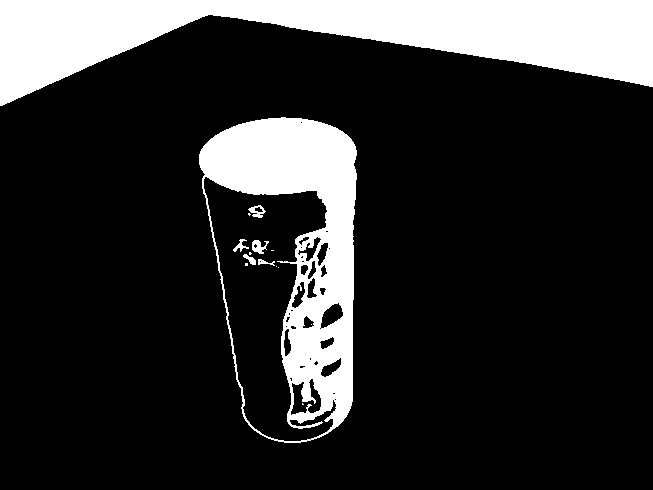
\includegraphics[width=0.14\textwidth]{interface/segmentation/2/re_2_pr_bgd.png}    & 					\hspace*{-13pt}
		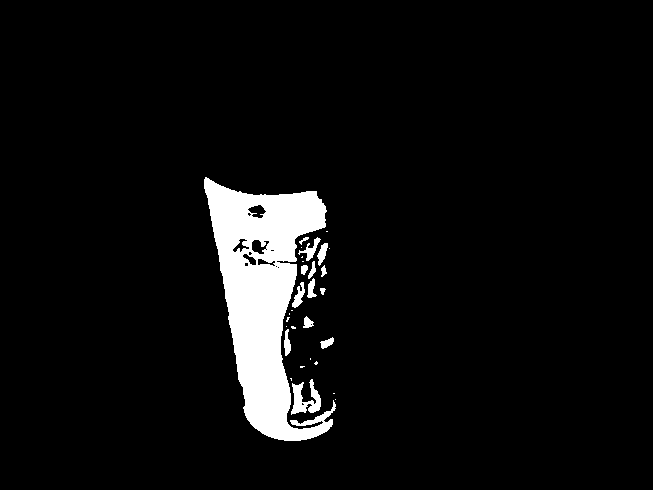
\includegraphics[width=0.14\textwidth]{interface/segmentation/2/re_2_pr_fgd.png}    & 					\hspace*{-13pt}
		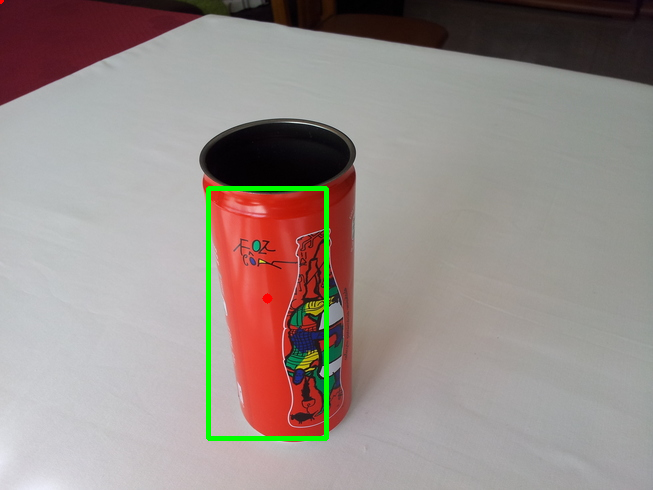
\includegraphics[width=0.14\textwidth]{interface/segmentation/2/re_2_rect.png}    & 					\hspace*{-13pt}
		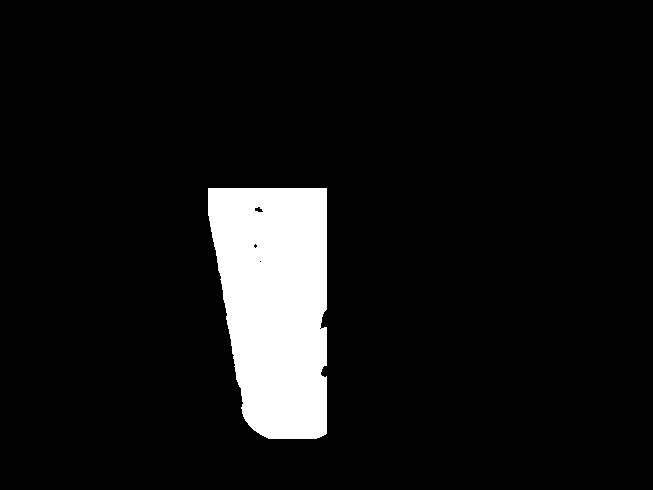
\includegraphics[width=0.14\textwidth]{interface/segmentation/2/re_2_mask.png}    & 					\hspace*{-13pt}
		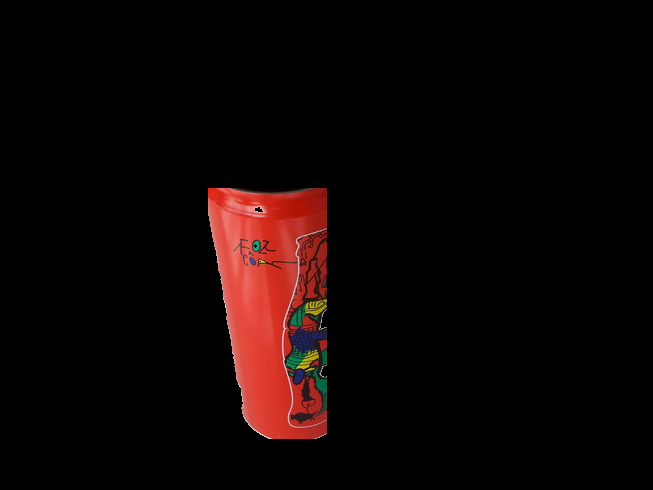
\includegraphics[width=0.14\textwidth]{interface/segmentation/2/re_2_seg.png} \\
                
    	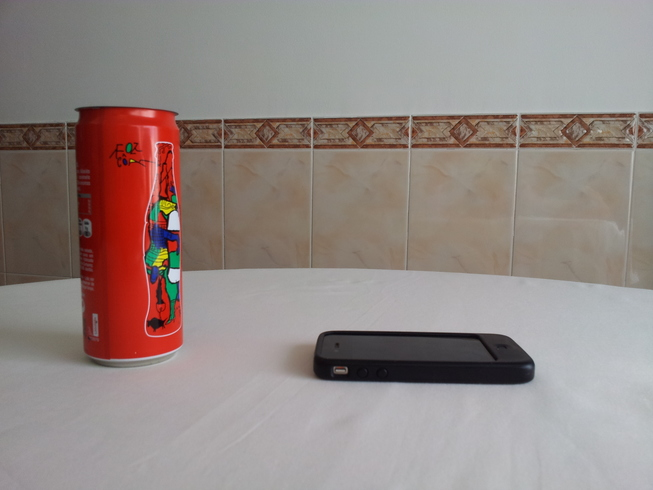
\includegraphics[width=0.14\textwidth]{interface/segmentation/4/re_4.jpg}    & 							\hspace*{-13pt}
		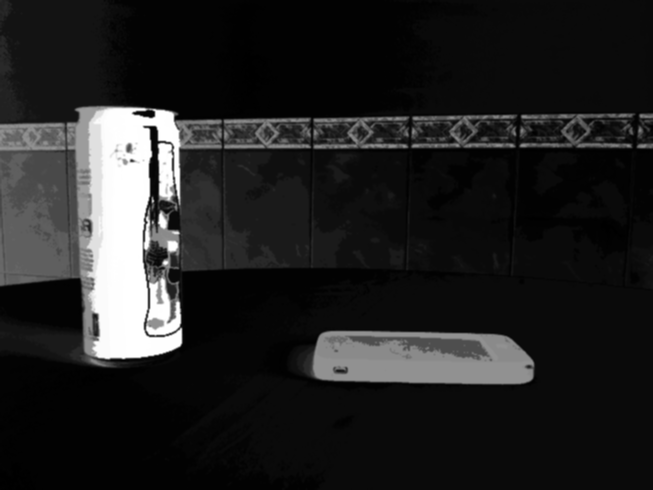
\includegraphics[width=0.14\textwidth]{interface/segmentation/4/re_4_sal.png}    & 						\hspace*{-13pt}
		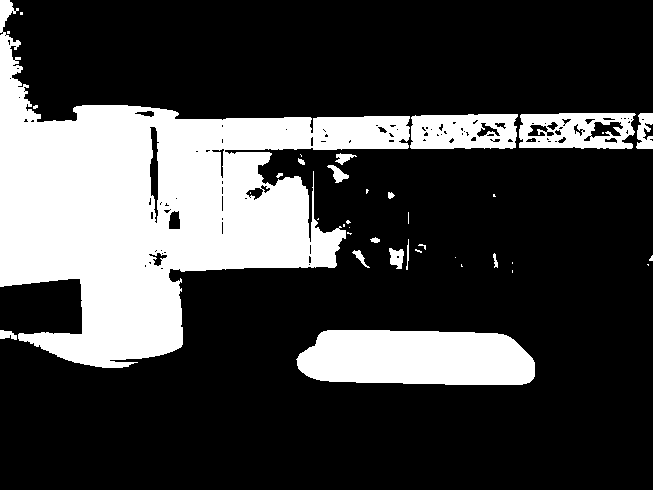
\includegraphics[width=0.14\textwidth]{interface/segmentation/4/re_4_bmask.png}    & 					\hspace*{-13pt}
		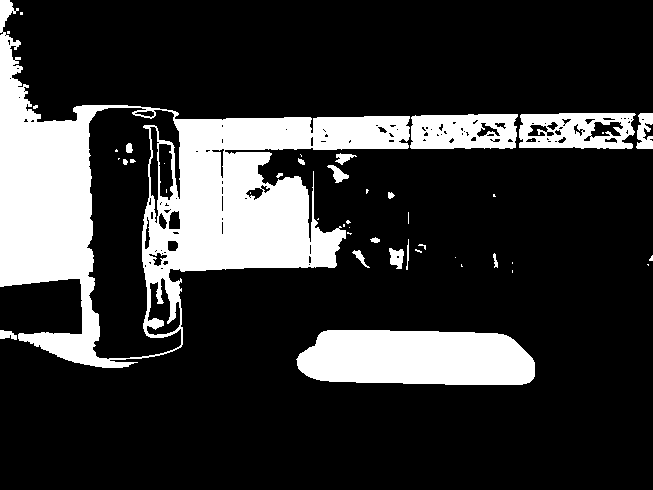
\includegraphics[width=0.14\textwidth]{interface/segmentation/4/re_4_pr_bgd.png}    & 					\hspace*{-13pt}
		
\includegraphics[width=0.14\textwidth]{interface/segmentation/4/re_4_pr_fgd.png}    & 					\hspace*{-13pt}
		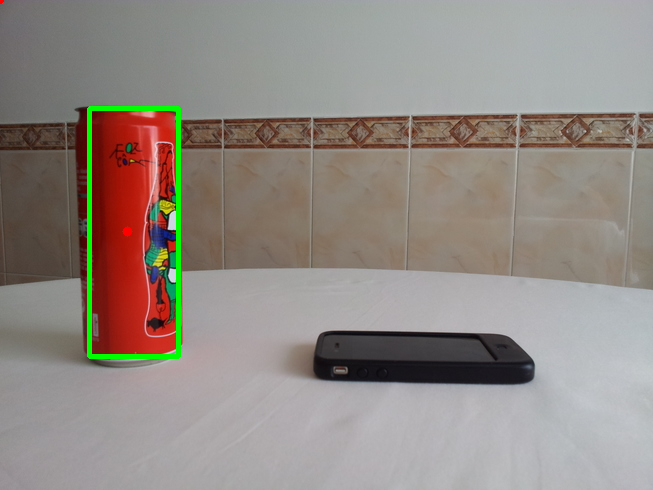
\includegraphics[width=0.14\textwidth]{interface/segmentation/4/re_4_rect.png}    & 					\hspace*{-13pt}
		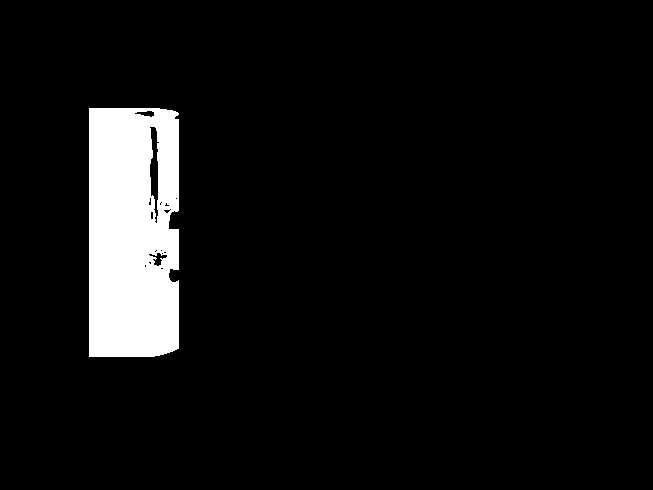
\includegraphics[width=0.14\textwidth]{interface/segmentation/4/re_4_mask.png}    & 					\hspace*{-13pt}
		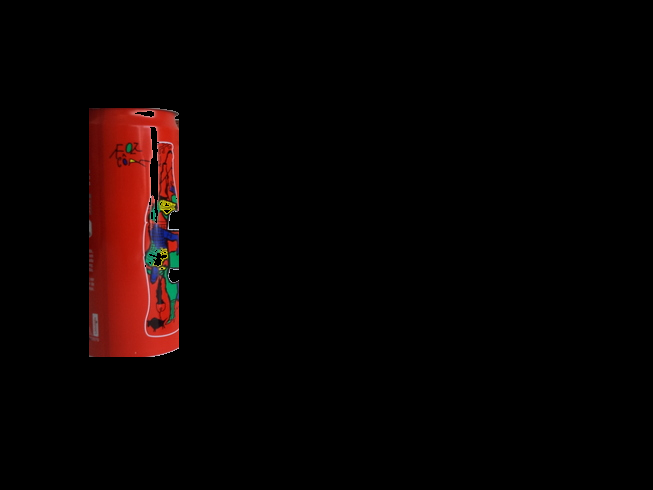
\includegraphics[width=0.14\textwidth]{interface/segmentation/4/re_4_seg.png} \\
		
		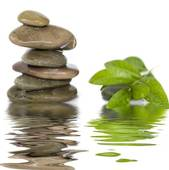
\includegraphics[width=0.14\textwidth]{interface/segmentation/10/10.jpg}        &
        \hspace*{-13pt}
		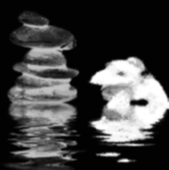
\includegraphics[width=0.14\textwidth]{interface/segmentation/10/10_sal.png}    & 						\hspace*{-13pt}		
		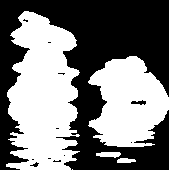
\includegraphics[width=0.14\textwidth]{interface/segmentation/10/10_bmask.png}    & 					\hspace*{-13pt}		
		
\includegraphics[width=0.14\textwidth]{interface/segmentation/10/10_pr_bgd.png}    & 					\hspace*{-13pt}		
		
\includegraphics[width=0.14\textwidth]{interface/segmentation/10/10_pr_fgd.png}    & 					\hspace*{-13pt}		
		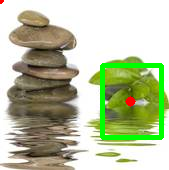
\includegraphics[width=0.14\textwidth]{interface/segmentation/10/10_rect.png}    & 						\hspace*{-13pt}		
		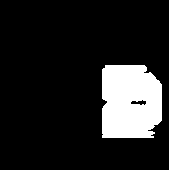
\includegraphics[width=0.14\textwidth]{interface/segmentation/10/10_mask.png}    &
		\hspace*{-13pt}		
		
\includegraphics[width=0.14\textwidth]{interface/segmentation/10/10_seg.png} \\
		
		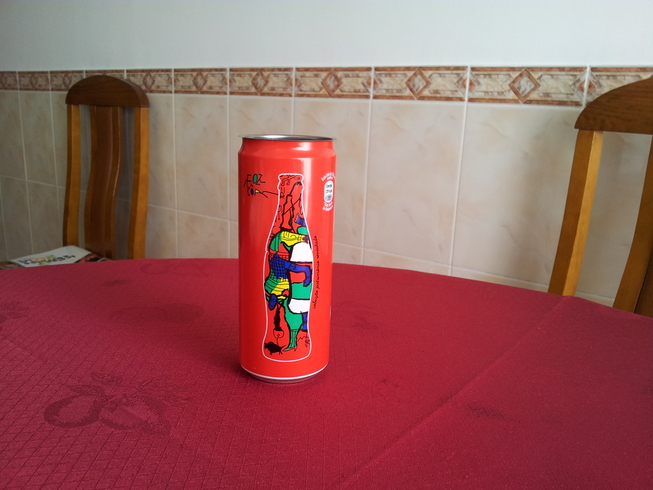
\includegraphics[width=0.14\textwidth]{interface/segmentation/7/re_7.jpg}        &
        \hspace*{-13pt}
		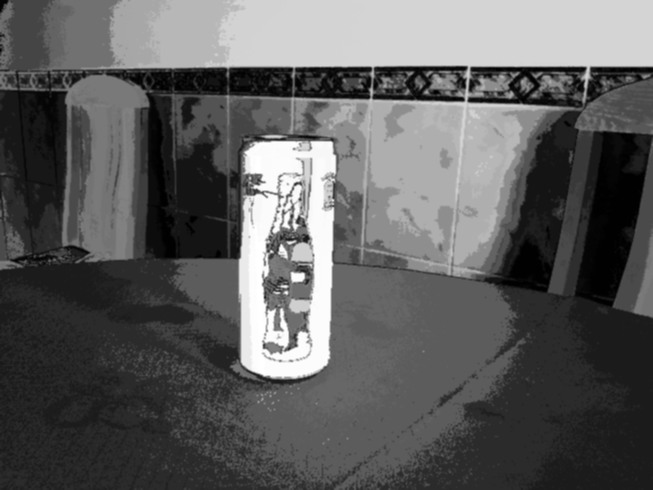
\includegraphics[width=0.14\textwidth]{interface/segmentation/7/re_7_sal.png}    & 						\hspace*{-13pt}		
		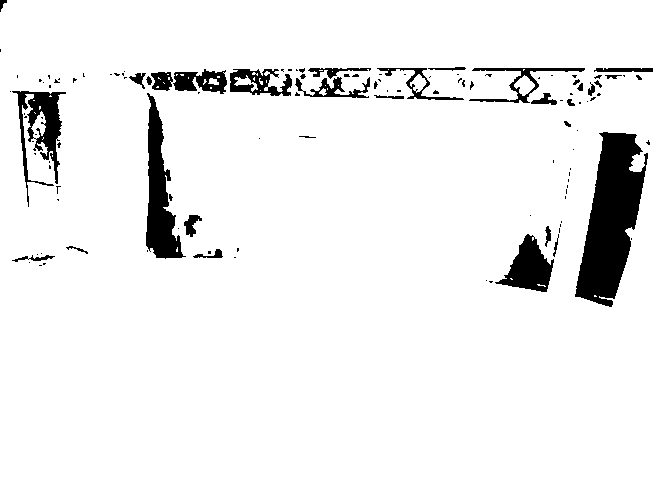
\includegraphics[width=0.14\textwidth]{interface/segmentation/7/re_7_bmask.png}    & 					\hspace*{-13pt}		
		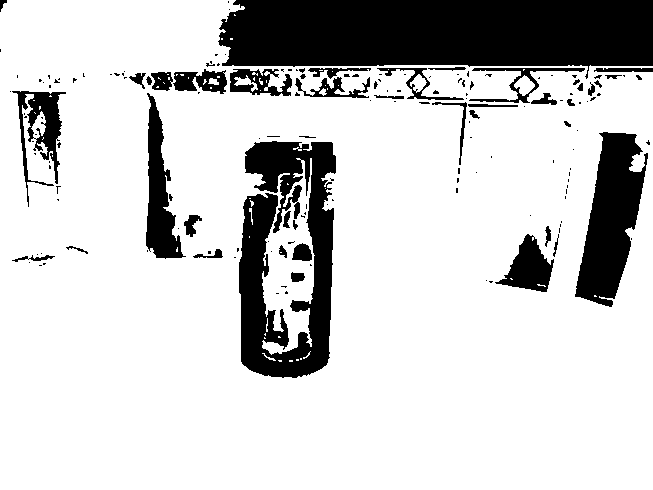
\includegraphics[width=0.14\textwidth]{interface/segmentation/7/re_7_pr_bgd.png}    & 					\hspace*{-13pt}		
		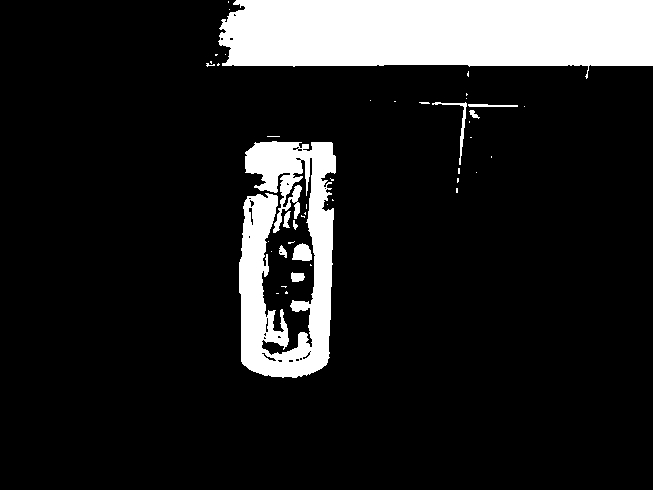
\includegraphics[width=0.14\textwidth]{interface/segmentation/7/re_7_pr_fgd.png}    & 					\hspace*{-13pt}		
		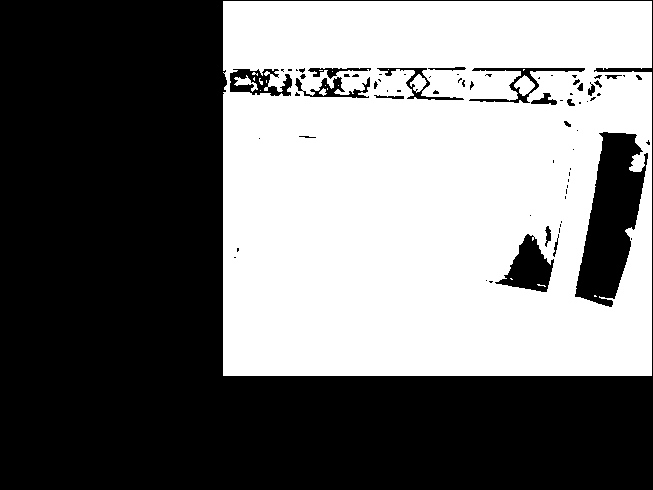
\includegraphics[width=0.14\textwidth]{interface/segmentation/7/re_7_mask.png}    & 					\hspace*{-13pt}		
		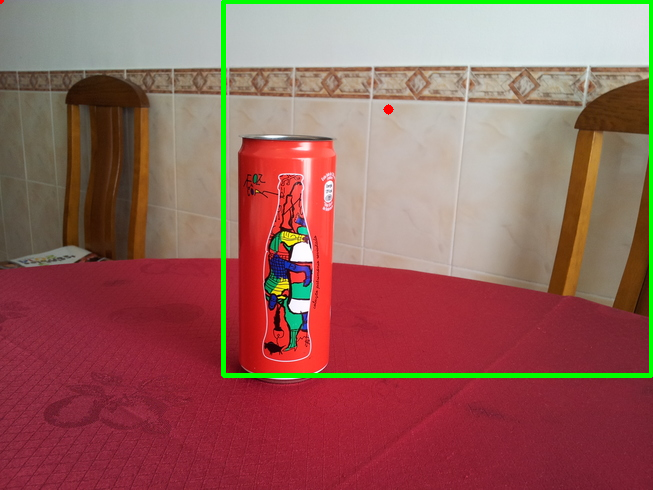
\includegraphics[width=0.14\textwidth]{interface/segmentation/7/re_7_rect.png}    &
		\hspace*{-13pt}		
		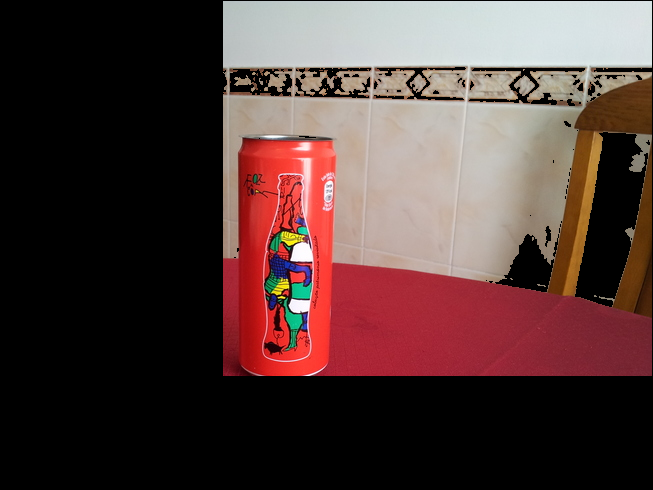
\includegraphics[width=0.14\textwidth]{interface/segmentation/7/re_7_seg.png} \\
		a) & \hspace*{-13pt} b) & \hspace*{-13pt} c) & \hspace*{-13pt} d) & \hspace*{-13pt} e) & \hspace*{-13pt} f) & \hspace*{-13pt} g) & \hspace*{-13pt} h)
    \end{tabular}
      \caption{Steps taken when segmenting an object. a) Input image. b) Saliency map generated by the algorithm in \cite{cheng2011global}. c) Binary mask. d) Probable background pixels. e) Probable foreground pixels. f) Bounding rectangle and center of mass point. g) Cropped mask containing the probable foreground area filled in with probable background pixels. h) Segmentation applied to the input image.}      
      
\end{figure}

Has it is possible to observe in Figure \ref{fig:seg_example}, the input image shows a singular object in a plain background with a successful segmentation. The second image it is possible to confirm that, although the object is detected, the foreground threshold is not sensitive to lightning changes, as the darkest side in the can is considered as being a probable background.

This algorithm also might not work when trying to segment two objects. Example of this is the third input image, where we can verify by the saliency map, that the can is obviously more salient than the other object, therefore, the second object is classified as probable background. Another example of this, is the fourth image. With a plain background and two objects, the object with more vivid colours is the one considered as foreground, leaving the remaining object as part of the foreground.

The fifth image shows an example were lightning changes affect the outcome of the algorithm. In this case, the can and a part of the wall are considered as foreground. The solution to this would be a higher threshold when defining the foreground pixels, as the wall is visibly less salient than the can in the saliency map. Since it is detecting the wall as a part of the foreground, this causes the center of mass to be slightly dislocated and generates a bigger bounding rectangle. When merging the probable foreground pixels with the probable background ones and cropping with the bounding rectangle, it segments a big portion of the image that its not relevant.

This object segmentation was also used in other functionalities implemented for this thesis.

\todo[inline]{fazer comparação com dataset utilizado no paper}
\subsection{Image Simplicity}
\label{sub:background}

To reduce the attention distraction by the objects in the background, professional photographers make the background simple. With that perspective in mind, the simplicity of a photo was considered a good feature to analyse.
The most easiest form to obtain simplicity is to place the subject against a neutral background like a backdrop or the sky. Backgrounds can be entirely neutral, like a solid backdrop or a cloudless sky; or they can complement the image, like a starfish on the sand.

Since snapshots often have cluttered backgrounds, professional photos are expected to have edges uniformly distributed in the image, as well, as a subject well defined and in focus. 


\subsubsection{Algorithm Description}

We experimented three algorithms that approach this problem. For our first experiment, we implemented an algorithm described in \cite{kaoautomatic}. Although very simple, the intuition behind this algorithm is that a very complex image, is likely to contain a large amount of edges. In \cite{kaoautomatic} only describes the feature as:

\begin{equation}
	B_{complexity} = \frac{n_{e}}{n_{T}},
\end{equation}
where $n_{e}$ is the number of pixels that are edge and $n_{T}$ is the total number of pixels.
 
 
The second algorithm that we tested was presented by \citeauthor{luo2008photo} in \cite{luo2008photo}, were the author explored the simplicity of a photo through its colour distribution.

As described in \cite{luo2008photo}, for a photo, we quantize each color of the RGB channels into 16 values, creating a histogram with 4096 bins, which gives the counts of quantized colors present in the image. After creating the histogram, we calculate the maximum count ($h_{max}$) in the histogram. The simplicity of a photograph is then defined as:
\begin{equation}
	Simplicity = (\|S\|/4096) * 100%,
\end{equation}
where $S$ is the number of bins in the histogram that equal or bigger than $\gamma h_{max}$. $\gamma$ is 0.01 as chosen by the author in the original article. As described in \cite{luo2008photo}, the simplicity factor for high quality photos fall in $[0\%,1.5\%]$, and low quality photos in $[0.5\%,5\%]$.

In our third experiment we implemented an algorithm described in \cite{ke2006design} by \citeauthor{ke2006design}, were the idea was to compute the spatial distribution of the high frequency edges. Since the snapshots often haven cluttered backgrounds, edges are expected to be uniformly distributed in the image. In professional photographs, the subject is normally well defined and in focus, meaning that high frequency edges will be placed in a smaller area.
We started by implementing a $3\times3$ Laplacian matrix with $\alpha = 0.2$ as follows:
\begin{equation}
\begin{bmatrix}
  0.2 & 0.8 & 0.2 \\
  0.8 & -4 & 0.8 \\
  0.2 & 0.8 & 0.8
\end{bmatrix}
\end{equation}

This is matrix is then applied to the image and take its absolute value to ignore the direction of the gradients. Since this algorithm is to be applied on coloured images in real-time, we split the channels of each frame and perform this computation on each channel, taking the mean across the channels in the end. This will create a Laplacian image that will be resized to $100\times100$ and normalized to values between 0 and 1. This will help when calculating the amount of area the edges occupy. It is expected for well defined objects as the ones used in high quality photos to produce a smaller bounding box, on the other hand cluttered images, are expected to have the oppose effect.
The area of the bounding box is calculated by projecting the Laplacian image $L$ onto de $x$ and $y$ axis independently so that:
\begin{equation}
P_{x}(i) = \sum_{y} L(i,y),
\end{equation}
\begin{equation}
P_{y}(j) = \sum_{x} L(x,j).
\end{equation}

This result in two vectors, one for $x$ axis and another one for $y$, that will have a length correspondent to the image width and height, were each position in the vector will have the amount of pixels considered as an edge in that column or row.

After the projection of the Laplacian image onto the $x$ and $y$ axis, we find the position with the largest count of edges for each vector. The position with the maximum count will be considered the peak and we calculate the width $w_{x}$ and $w_{y}$ for each vector, that contains 98\% of the mass of the projections $P_{x}$ and $P_{y}$. The area of the bounding box containing a high density of pixels is then defined by $w_{x}w_{y}$ and the quality measure for the image is then $1-w_{x}w_{y}$.

\subsubsection{Interface Display}

In our application we tried to understand how these three algorithms would perform under a scenario were this feature would be used in real-time. For that we displayed on the screen the scores obtained from each method were, for the first algorithm\cite{kaoautomatic} and third algorithm\cite{ke2006design}, the score is between 0 and 1, and greater values indicate a simplicity in the scenario. 
For the algorithm presented in \cite{luo2008photo}, can obtain any value between 0\% and 100\% but the author considers a photo simple if the score is between 0.5\% and 5\%. An example of the visualization of these scores can be seen in Figure X.

\todo[inline]{Screenshot a mostrar os scores de simplicidade}

Alternatively, these scores could be replaced a bar that represents the full scale of each algorithm with a marker indicating the current score of the frame.

\todo[inline]{Screenshot a mostrar os scores de simplicidade em barras}

\subsubsection{Discussion}



\subsection{Main Line Detection}
\label{sub:line_detection}

Lines can have an important role in a photograph, as referred in \ref{subsub:leading_lines}. These lines can have multiple interpretations, depending if they are horizontal, vertical, diagonal or curved. They can give a sensation of stability and safety, movement or delimit the begin and the end of a scene.

A popular method for edge detection is the use of Canny Edge Detector\cite{canny1986computational} which can detect the main edges of an image. This method is applies several convolution filters to each pixel with the goal of finding the pixels where the intensity variation is high\cite{nobrega2013interactive}.
The algorithm starts by applying a Gaussian filter which will blur the image reducing the noise and extra edges that might be detected. After the Gaussian filter, it applies two Sobel kernels to find gradients in the horizontal and vertical direction such as:
\begin{equation}
S_{x} =
\begin{bmatrix}
	-1 & 0 & 1\\
	-2 & 0 & 2\\
	-1 & 0 & 1
\end{bmatrix}
,
S_{y} = 
\begin{bmatrix}
	-1 & -2 & -1\\
	0 & 0 & 0\\
	1 & 2 & 1
\end{bmatrix}
\end{equation}
Finally the gradient of a pixel is calculated by
\begin{equation}
	S_{p} = \sqrt{S_{x}^{2} + S_{y}^{2}},
\end{equation}
and the pixel will be accepted as an edge if it is above an upper threshold, below the lower threshold or connected to a pixel that is above the upper threshold.

Another method of line detection used is the through the Hough Transformation\cite{illingworth1988survey}. Lines can be represented in the Cartesian space by the equation
\begin{equation}
	y=mx+b.
	\label{eq:recta}
\end{equation}

Any line can be represented by the equation \ref{eq:recta} and therefore, it can be manipulated to other coordinates such as Polar Coordinates, where its general equation would be
\begin{equation}
	y=\left( -\frac{cos \theta}{sin \theta} \right) x + \left(\frac{r}{sin \theta}\right),
\end{equation}
and peach point on a plane is determined by a distance $r$ from a fixed point and an angle $\theta$ from a fixed direction.
The Hough Transform consists in a two-dimensional space where each line is represented by a tuple $(r,\theta)$ and therefore all lines can be represented in the Hough Space by the equation
\begin{equation}
r = x_{0}cos\theta + y_{0}sin\theta.
\end{equation}
The combination of the Canny Edge detector and the representation of a line in the Hough Space will be useful in the implementation of this functionality.

\subsubsection{Algorithm Description}
\subsubsection{Interface Display}
\subsubsection{Discussion}

\subsection{Horizon Detection}
\label{sub:horizon_detection}

\subsection{Image Balance}
\label{sub:balance}

\section{Discussion}
\label{sec:system_discussion}